\section{Change of Variables: Jacobians}\label{sec:Jacobian}

In sections \ref{sec:double_int_polar} and \ref{sec:cylindrical_spherical} we learned how to set up and evaluate integrals in coordinate systems other than the familiar rectangular coordinate system.  In each of these cases, we observed that changing coordinate systems could make it much easier to evaluate a double or triple integral because the descriptions of the regions of integration were much simpler using a more appropriate coordinate system.

Recall that this process of integrating in a new coordinate system involves more than simply using formulas to change variables: $x = r\cos \theta$ and $y = r\sin \theta$ for the polar and cylindrical coordinate systems and $x = \rho\sin\varphi \cos \theta, y = \rho\sin\varphi\sin\theta$ and $z = \rho\cos\varphi$ for the spherical coordinate system.  In polar coordinates, $dA$ becomes $r\,drd\theta$, in cylindrical coordinates, $dV$ becomes $r\,dzdrd\theta$, and in spherical coordinates $dV$ becomes $\rho^2\sin\varphi \,d\rho d\theta d\varphi.$  We derived these descriptions using geometric ideas and carefully drawn pictures.  In this section, we learn a general technique for converting integrals between coordinate systems.\\

\noindent\textbf{\large Motivation Using Integrals In One Dimension.}\\

Suppose we want to evaluate the definite integral
\[
	\int_0^3 x\sqrt{1+x^2}\,dx.
\]
Using the substitution $u= 1+x^2$, we calculate the differential $du = 2x\,dx$ and update the limits of integration to find
\[
	\int_0^3 x\sqrt{1+x^2}\,dx = \frac{1}{2}\int_1^{10} \sqrt{u}\,du.
\]
The second integral is easier to evaluate due to the significant simplification of the integrand.  We can describe the ``$u$-substitution'' process as a more general change of variables process.  Define $x = g(u)$.  Then $dx = g'(u)\,du$, and we can write
\[
	\int_a^b f(x)\,dx = \int_c^d f(g(u))g'(u)\,du,
\]
where $a = g(c)$ and $b = g(d)$.  Using this slightly different formulation in our integral, we have $x = \sqrt{u-1}$ and $dx = \frac{1}{2\sqrt{u-1}}\,du.$  Then
\[
	\int_0^3 x\sqrt{1+x^2}\,dx = \int_1^{10} \sqrt{u-1}\sqrt{u}\frac{1}{2\sqrt{u-1}}\,du =  \frac{1}{2}\int_1^{10} \sqrt{u}\,du.
\]

Though different than our usual way of performing a $u$-substitution, this modified formulation has the benefit of clearly demonstrating that three things change in the integral when we switch from one variable to a different variable.  First, the region of integration changes.  In this case, that means the interval changes, but for higher dimensions, this corresponds to a change in a higher dimensional region.  Second, the integrand changes.  Third, the $dx$ changes.  In two or three dimensions, this corresponds to a change in $dA$ and $dV.$ In the context of higher dimensional problems, we may desire to focus on the first change.  In other words, we may wish to change coordinates in an effort to simplify a complicated region of integration.  Alternatively, we may have an integral with a complicated integrand.  With the right change of variables, we may be able to work in a new coordinate system that significantly simplifies the integrand.  In the pages that follow, we describe the general process of changing variables.  For simplicity, we focus exclusively on two dimensional problems.\\

\noindent\textbf{\large Transformations}\\

Consider the change of variables given by
\[
	x = f(u,v) \text{ and } y = g(u,v).
\]
Define the function
\[
	T(u,v) = (x,y) = (f(u,v),g(u,v)).
\]
We call $T$ a transformation from the $uv$-plane to the $xy$-plane.  Given a point $(u_1,v_1)$ in the $uv$-plane, the transformation $T$ returns a point $(x_1,y_1)$ in the $xy$-plane with coordinates $(f(u_1,v_1),g(u_1,v_1)).$  If the functions $f$ and $g$ are one-to-one, the inverse transformation $T\primeskip^{-1}$ transforms the point $(x_1,y_1)$ in the $xy$-plane into the point $(u_1,v_1)$ in the $uv$-plane.

For regions, $T$ transforms the region $S$ in the $uv$-plane into the region $R$ in the $xy$-plane, and $T\primeskip^{-1}$ transforms the region $R$ in the $xy$-plane into the region $S$ in the $uv$-plane.  These ideas are shown graphically in figure \ref{fig:transformation}

%\mfigure{.8}{Visualization of the transformation $T$.}{fig:transformation}{figures/fig12_Jacobian_transformation}

% because middle of the page figures get labels before the marginal ones do, we need to adjust the figure
% count.
\addtocounter{figure}{1}
\vskip 10pt
\hskip-50pt
\noindent\begin{minipage}[t]{\textwidth+100pt}
	\begin{tabular}{ccc}
		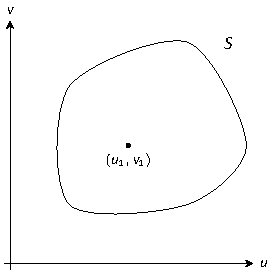
\includegraphics[align=c]{figures/fig13_jacobian_transformation_a} & 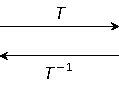
\includegraphics[align=c]{figures/fig13_jacobian_transformation_c} & 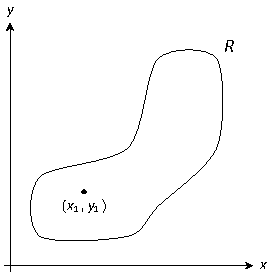
\includegraphics[align=c]{figures/fig13_jacobian_transformation_b}
	\end{tabular}
	\captionsetup{type=figure}%
	\caption{Visualization of the transformation $T$.}
	\label{fig:transformation}
\end{minipage}
\\
\vskip10pt
% further adjusting figure count
\addtocounter{figure}{-2}

\example{ex_transform_box}{Transforming a Rectangle}{
	Consider the transformation $T(u,v)$ defined by
	\begin{align*}
		x &= u^2\\
		y &= u + v.
	\end{align*}
	Let $S$ be the rectangular region in the $uv$-plane bounded by the lines 
	\[
		u=1, u=2, v=0, \text{ and } v=6.
	\]
	Describe the transformed region $R$ in the $xy$-plane.}
{We first consider the bottom side of the rectangle given by $v=0$ and $1 \leq u \leq 2.$  Using the transformation $T$, we have $x = u^2$ and $y=u + 0.$ Combining, we see that the base of the rectangle in the $uv$-plane transforms into the curve $y = \sqrt{x}$ for $1 \leq x \leq 4$ in the $xy$-plane.
	
The top side of the rectangle in the $uv$-plane is given by $v=6$ and $1 \leq u \leq 2.$  Using the transformation $T$, we now have $x=u^2$ and $y=u+6.$  Combining, the top of the rectangle in the $uv$-plane transforms into the curve $u = \sqrt{x}+6$ for $1 \leq x \leq 4.$

For the left side of the rectangle in the $uv$-plane, we have $u=1$ and $0 \leq v \leq 6.$  The transformation $T$ gives $x = 1$ and $y = 1+v$.  This is the vertical line segment $x=1$ and $1 \leq y \leq 7.$

The right side of the rectangle in the $uv$-plane is given by $u=2$ and $0 \leq v \leq 6.$ The transformation $T$ gives $x = 4$ and $y = 2 + v$, yielding the vertical line segment $x=4$ and $2 \leq y \leq 8.$

The the original region $S$ in the $uv$-plane and the transformed region $R$ in the $xy$-plane are shown in figure~\ref{fig:transform_box}.
}

\mtable{.65}{The regions $S$ and the transformed region $R$ from example~\ref{ex_transform_box}.}{fig:transform_box}{%
	\begin{tabular}{c}
		\myincludegraphics[scale=1]{figures/fig13_jacobian_transform_box_a}\\
		(a)\\[15pt]
		\myincludegraphics[scale=1]{figures/fig13_jacobian_transform_box_b}\\
		(b)
	\end{tabular}
}

\vskip \baselineskip

Often, instead of starting with a region in the $uv$-plane and a transformation, we start with a region in the $xy$-plane and seek a transformation that transforms a simple region in the $uv$-plane into the given region in the $xy$-plane.  We work through this process in the next example.

\vskip \baselineskip

\example{ex_transform_parallelogram}{Transforming a Rectangle into a Parallelogram}{
	Find a change of variables that transforms a rectangular region in the $uv$-plane into the parallelogram shown in figure~\ref{fig:transform_parallelogram}.}
{We first note that the region is bounded by the lines
	\begin{align*}
		4y - x &= 0\\
		4y - x &= 10\\
		2y - 3x &= 0\\
		2y - 3x &= -10.
	\end{align*}
The equations $4y-x=0$ and $4y-x=10$ describe the bottom and top edges of the parallelogram.  In general, the equation $4y-x = k$, for $0 \leq k \leq 10$, describes a family of parallel lines in the $yx$-plane that are parallel to the top and bottom edges of the parallelogram. These lines ``fill in" the parallelogram.  Similarly, the equation $2y-3x=p$, for $-10 \leq p \leq 0$, describes a family of lines in the $xy$-plane that are parallel to the right and left edges of the parallelogram and ``fill in" the parallelogram.

These observations suggest the change of variables $u = 4x-y$ and $v = 2y-3x$ where $0 \leq u \leq 10$ and $-10 \leq v \leq 0.$  Notice though that this is not the transformation we seek.  We want a transformation $T$ that maps the $uv$-plane into the $xy$-plane.  The change of variables suggested maps the $xy$-plane into the $uv$-plane.  Instead of describing $T$, the change of variables defines the inverse transformation, $T^{\primeskip -1}.$  To find $T$, we must solve for $x$ and $y$.  Working through this algebraic process yields the transformation $T(u,v)$ defined by
	\begin{align*}
		x &= \frac{u-2v}{5}\\
		y &= \frac{3u-v}{10}
	\end{align*}
This transformation maps the rectangular region $0 \leq u \leq 10$ and $-10 \leq v \leq 0$ in to the parallelogram shown in figure~\ref{fig:transform_parallelogram}.
}

\mfigure{.8}{The transform from example \ref{ex_transform_parallelogram} transforms a rectangular region in the $uv$-plane into the parallelogram shown above.}{fig:transform_parallelogram}{figures/fig13_jacobian_transform_parallelogram}

\noindent\textbf{\large The Change of Variables Theorem for Double Integrals}\\

We have seen how transformations affect regions.  We need to know how they affect integrals.  Consider a small rectangle $S$ in the $uv$-plane with side length $\Delta u$ and $\Delta v.$  This rectangle is transformed by the transformation $T(u,v) = (f(u,v),g(u,v))$ into the region $R$ in the $xy$-plane as shown below.

% because middle of the page figures get labels before the marginal ones do, we need to adjust the figure
% count.
\addtocounter{figure}{1}
\vskip 10pt
\hskip-50pt
\noindent\begin{minipage}[t]{\textwidth+100pt}
	\begin{tabular}{ccc}
		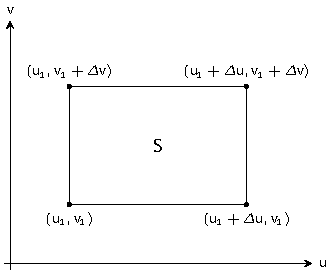
\includegraphics[align=c]{figures/fig13_jacobian_area_transformation_a} & 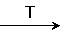
\includegraphics[align=c]{figures/fig13_jacobian_area_transformation_b} & 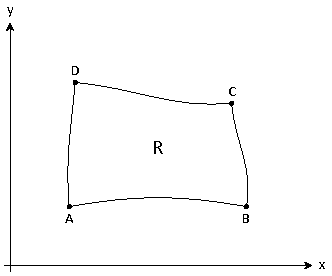
\includegraphics[align=c]{figures/fig13_jacobian_area_transformation_c}
	\end{tabular}
	\captionsetup{type=figure}%
	\caption{A small region transformed by $T(u,v) = (f(u,v),g(u,v))$.  The transformed points have coordinates $A = (f(u_1,v_1),g(u_1,v_1)), B = (f(u_1+\Delta u, v_1), g(u_1+\Delta u, v_1)), C = (f(u_1+ \Delta u,v_1 + \Delta v), g(u_1 + \Delta u, v_1 + \Delta v)),$ and $D = (f(u_1,v_1 + \Delta v),g(u_1, v_1 + \Delta v)).$}
	\label{fig:area_transformation}
\end{minipage}
\\
\vskip10pt
% further adjusting figure count
\addtocounter{figure}{-2}

The vector $\vv{AB}$ in figure \ref{fig:area_transformation} is given by \[\vv{AB}~=~\langle f(u_1+\Delta u,v_1)-f(u_1,v_1),g(u_1+\Delta u,v_1)-g(u_1,v_1)\rangle.\]  Similarly, \[\vv{AD} = \langle f(u_1,v_1 + \Delta v) - f(u_1,v_1), g(u_1,v_1 + \Delta v) - g(u_1,v_1)\rangle.\]  Recall that the magnitude of the cross product $||\vv{AB} \times \vv{AD}||$ gives the area of a parallelogram with sides $\vv{AB}$ and $\vv{AD}.$  It follows that the area of the transformed region $R$ is approximately equal to $||\vv{AB} \times \vv{AD}||.$


%\printexercises{exercises/13_06_exercises}